 \providecommand{\main}{../../..}
\documentclass[\main/main.tex]{subfiles}
\begin{document}
\subsection{Esercizio 1}
Dato il seguente problema di PL, si risolva graficamente e si ottenga il valore della soluzione ottima e di tutte le variabili di scarto.

Si ricavi, per via grafica, per quali valori di $c_2$, inizialmente pari a $-1$, la \textbf{composizione} della base ottima non cambia.

\begin{figure}
  \begin{align*}
    \max z = 2x_1 - x_2         \\
    x_1 + 2x_2 & \leq 4         \\
    2x_1 + x_2 & \geq 2         \\
    x_1 - 2x_2 & \leq 6         \\
    x_1        & \geq 0         \\
    x_2        & \in \mathbb{R}
  \end{align*}
  \caption{Esercizio 1}
\end{figure}

\subsection{Soluzione esercizio 1}

\subsubsection*{Disegno l'area di definizione del problema}
\begin{figure}
  \begin{subfigure}{0.45\textwidth}
    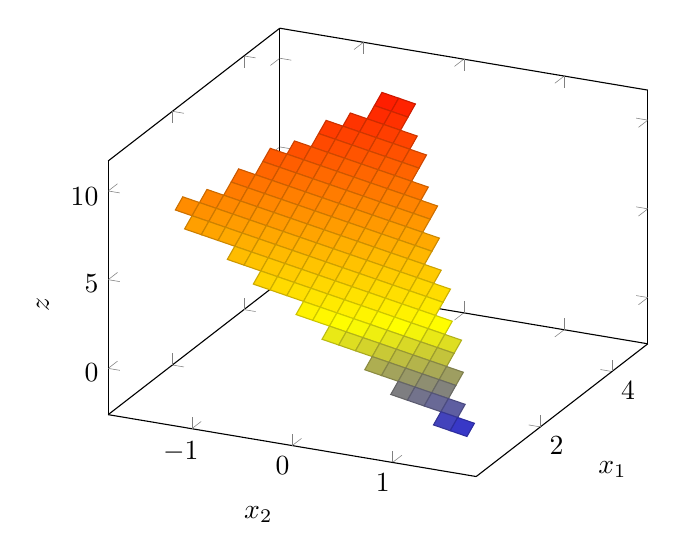
\begin{tikzpicture}
      \begin{axis}[
          xlabel=$x_2$,
          ylabel=$x_1$,
          zlabel=$z$,
          domain=-2:2,
          y domain=0:5
        ]
        \addplot3[surf, unbounded coords=jump]
        {
          y+2*x<=4 &&
          2*y +x >= 2 &&
          y -2*x <= 6 ?
          2*y-x:NaN
        };
      \end{axis}
    \end{tikzpicture}
    \caption{La funzione $z$}
  \end{subfigure}
  \begin{subfigure}{0.45\textwidth}
    \includegraphics[width=0.8\textwidth]{2016_11_16}
    \caption{Regione di definizione del problema}
  \end{subfigure}
\end{figure}

\subsubsection*{Identifico il punto di massimo}
Il punto di massimo si trova all'intersezione tra primo e terzo vincolo:
\[
  \begin{cases}
    x_1 + 2x_2 = 4 \\
    x_1 - 2x_2 = 6
  \end{cases}
  \Rightarrow
  \begin{cases}
    x_2 = -\frac{1}{2} \\
    x_1 = 5
  \end{cases}
\]

\begin{align*}
  z   = \frac{21}{2}  ,\quad
  x_1 = 5             ,\quad
  x_2 = -\frac{1}{2}  ,\quad
  s_1 = 0             ,\quad
  s_2 = -\frac{15}{2} ,\quad
  s_3 = 0
\end{align*}

\subsubsection*{Analisi di sensitività}
Al variare di $c_2$ posso spostare la soluzione ottima da $\rnd{5, -\frac{1}{2}}$ negli altri due vertici:

\paragraph*{Sposto soluzione ottima in $(2,-2)$:}

\[
  2(2) + c_2(-2) = 2(5) + c_2(-\frac{1}{2}) \Rightarrow c_2 = -4
\]
\paragraph*{Sposto soluzione ottima in $(0,2)$:}

\[
  2(0) + c_2(2) = 2(5) + c_2(-\frac{1}{2}) \Rightarrow c_2 = 4
\]


\begin{figure}
  \begin{subfigure}{0.45\textwidth}
    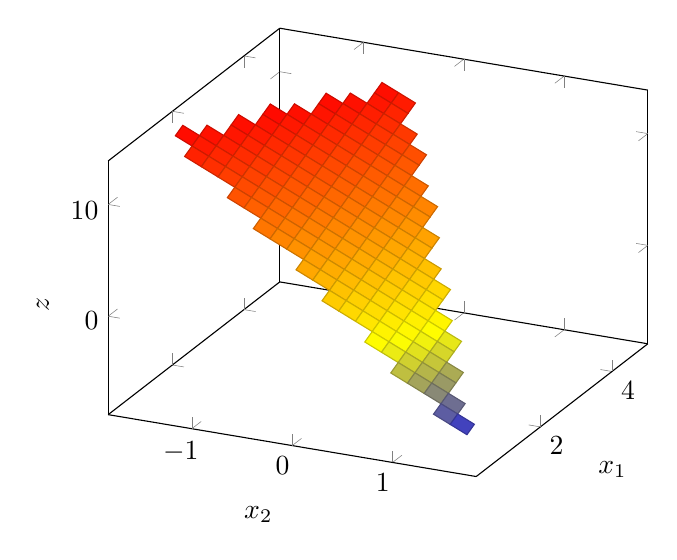
\begin{tikzpicture}
      \begin{axis}[
          xlabel=$x_2$,
          ylabel=$x_1$,
          zlabel=$z$,
          domain=-2:2,
          y domain=0:5
        ]
        \addplot3[surf, unbounded coords=jump]
        {
          y+2*x<=4 &&
          2*y +x >= 2 &&
          y -2*x <= 6 ?
          2*y-4*x:NaN
        };
      \end{axis}
    \end{tikzpicture}
    \caption{Sostituisco $c_2 = -4$}
  \end{subfigure}
  \begin{subfigure}{0.45\textwidth}
    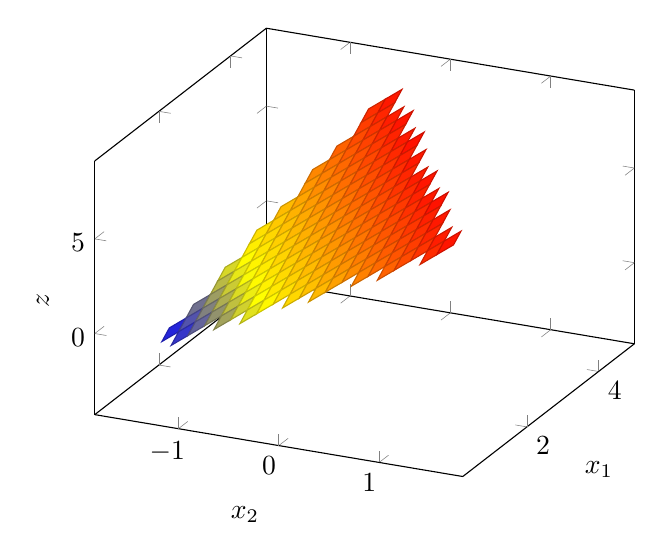
\begin{tikzpicture}
      \begin{axis}[
          xlabel=$x_2$,
          ylabel=$x_1$,
          zlabel=$z$,
          domain=-2:2,
          y domain=0:5
        ]
        \addplot3[surf, unbounded coords=jump]
        {
          y+2*x<=4 &&
          2*y +x >= 2 &&
          y -2*x <= 6 ?
          2*y+4*x:NaN
        };
      \end{axis}
    \end{tikzpicture}
    \caption{Sostituisco $c_2 = 4$}
  \end{subfigure}
  \caption{Analisi di Sensitività}
\end{figure}

\subsubsection*{Problema duale}

\begin{align*}
  \min z_D =  4y_1 + 2y_2 + 6y_3 \\
  y_1 + 2y_2 + y_3  & \geq 2     \\
  2y_1 + y_2 - 2y_3 & = -1       \\
  y_1, y_3          & \geq 0     \\
  y_2               & \leq 0
\end{align*}
\subsubsection*{Scarti complementari}
\[
  \begin{cases}
    x_1(y_1 + 2y_2 + y_3 - 2) = 0 \\
    x_2(2y_1 + y_2 - 2y_3 +1) = 0 \\
    y_1(x_1 + 2x_2 - 4) = 0       \\
    y_2(2x_1 + x_2 - 2) = 0       \\
    y_3(x_1 - 2x_2 - 6) = 0       \\
  \end{cases}
  \Rightarrow
  \begin{cases}
    y_1  + y_3 - 2 = 0 \\
    2y_1 - 2y_3 +1 = 0 \\
    y_2 = 0            \\
  \end{cases}
  \Rightarrow
  \begin{cases}
    y_1 = 2-y_3            \\
    2(2-y_3) - 2y_3 +1 = 0 \\
    y_2 = 0                \\
  \end{cases}
  \Rightarrow
  \begin{cases}
    y_1 = 2-y_3  \Rightarrow \frac{3}{4} \\
    y_3 = \frac{5}{4}                    \\
    y_2 = 0                              \\
  \end{cases}
\]
Verifico la soluzione ottima del duale: $z = z_D = \frac{21}{2}$

\end{document}